\section{Step Signal as $f(t)$}
For this analysis, we choose the \textbf{unit step function} as the input signal:

\begin{equation}
f(t) = u(t) = 
\begin{cases} 
1, & t \geq 0 \\
0, & t < 0 
\end{cases}
\end{equation}

\subsubsection{Interpretation:}
\begin{itemize}
    \item The output \( y(t) \) represents how the shape of \( f(t) \) is modified by \( h(t) \).
    \item The rectangular kernel \( h(t) \) acts as a moving average filter.
\end{itemize}

\subsection{Solution Using Step Function}

\subsubsection{Standard Convolution \( y(t) = (f * h)(t) \)}

Given:
\begin{itemize}
    \item \( f(t) = u(t) \) (step function)
    \item \( h(t) \) is a rectangular pulse centered at \( t = 0 \) with width \( 2T \).
\end{itemize}

The convolution integral is evaluated in three regions:

\begin{enumerate}
    \item \textbf{For \( t < -T \):}
    \begin{itemize}
        \item The kernel \( h(t - \tau) \) and \( u(\tau) \) do not overlap.
        \item Thus:
    \end{itemize}
    
    \begin{align}
        y(t) &= \int_{-\infty}^{\infty} u(\tau) h(t - \tau) \, d\tau \\
        &= \int_{0}^{\infty} 1 \cdot h(t - \tau) \, d\tau \\
        &= 0 \quad \text{(No overlap when $t < -T$)}
    \end{align}
    
    \item \textbf{For \( -T \leq t \leq T \):}
    \begin{itemize}
        \item The kernel partially overlaps \( u(\tau) \) from \( \tau = 0 \) to \( \tau = t + T \).
    \end{itemize}
    
    \begin{align}
        y(t) &= \int_{-\infty}^{\infty} u(\tau) h(t - \tau) \, d\tau \\
        &= \int_{0}^{\infty} 1 \cdot h(t - \tau) \, d\tau \\
        &= \int_{0}^{t+T} 1 \cdot 1 \, d\tau \quad \text{(Since $h(t-\tau)=1$ when $-T \leq t-\tau \leq T$)} \\
        &= [{\tau}]_{0}^{t+T} \\
        &= t + T
    \end{align}
    
    \item \textbf{For \( t > T \):}
    \begin{itemize}
        \item The kernel fully overlaps \( u(\tau) \) over a width of \( 2T \).
    \end{itemize}
    
    \begin{align}
        y(t) &= \int_{-\infty}^{\infty} u(\tau) h(t - \tau) \, d\tau \\
        &= \int_{0}^{\infty} 1 \cdot h(t - \tau) \, d\tau \\
        &= \int_{t-T}^{t+T} 1 \, d\tau \quad \text{(Since $h(t-\tau)=1$ when $t-T \leq \tau \leq t+T$)} \\
        &= [{\tau}]_{t-T}^{t+T} \\
        &= (t+T) - (t-T) \\
        &= 2T
    \end{align}
\end{enumerate}

\textbf{Final Result:}
\begin{equation}
y(t) = 
\begin{cases} 
0, & t < -T \\
t + T, & -T \leq t \leq T \\
2T, & t > T 
\end{cases}
\end{equation}

\subsubsection{Behavior Analysis:}
\begin{itemize}
    \item The output is zero before \( t = -T \).
    \item A linear ramp occurs from \( t = -T \) to \( t = T \).
    \item The output saturates at \( 2T \) for \( t > T \).
    \item A larger \( T \) results in a wider ramp and higher saturation value.
\end{itemize}
Here is plot showing the results
\begin{figure}[H]
    \centering
    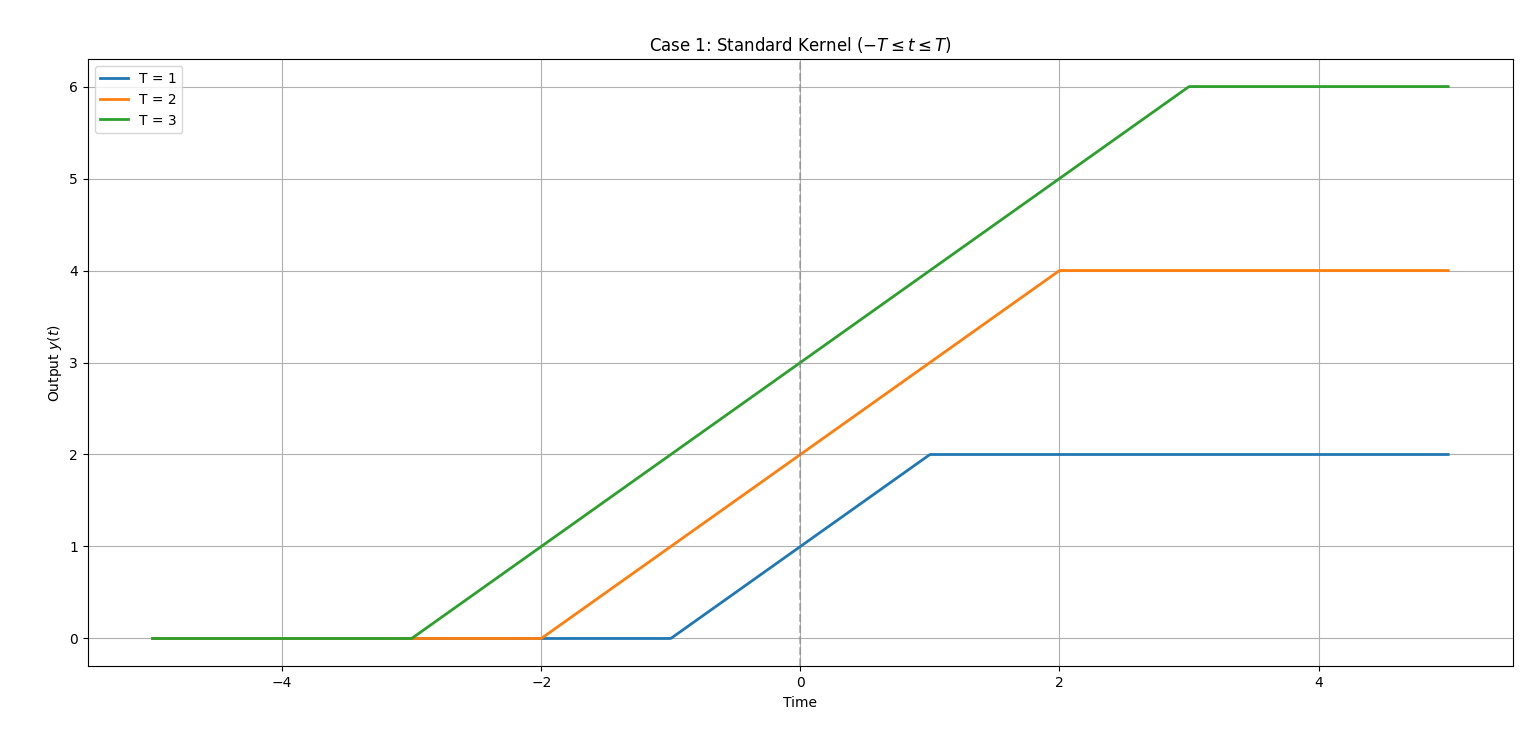
\includegraphics[width=0.8\linewidth]{codes/codes_step/plotsstep/case1step.png}
    \label{fig:enter-label}
\end{figure}
\subsubsection{Modified Kernel (Only \( t > 0 \)) (Part a)}

The modified kernel is:
\begin{equation}
h_{mod}(t) = 
\begin{cases} 
1, & 0 \leq t \leq T \\
0, & \text{otherwise}
\end{cases}
\end{equation}

\textbf{Convolution Analysis:}

\begin{enumerate}
    \item \textbf{For \( t < 0 \):}
    \begin{align}
        y(t) &= \int_{-\infty}^{\infty} u(\tau) h_{mod}(t - \tau) \, d\tau \\
        &= 0 \quad \text{(No overlap when $t < 0$)}
    \end{align}
    
    \item \textbf{For \( 0 \leq t \leq T \):}
    \begin{align}
        y(t) &= \int_{-\infty}^{\infty} u(\tau) h_{mod}(t - \tau) \, d\tau \\
        &= \int_{0}^{t} 1 \cdot 1 \, d\tau \quad \text{(Overlap from $\tau = 0$ to $\tau = t$)} \\
        &= [{\tau}]_{0}^{t} \\
        &= t
    \end{align}
    
    \item \textbf{For \( t > T \):}
    \begin{align}
        y(t) &= \int_{-\infty}^{\infty} u(\tau) h_{mod}(t - \tau) \, d\tau \\
        &= \int_{t-T}^{t} 1 \cdot 1 \, d\tau \quad \text{(Full overlap from $\tau = t-T$ to $\tau = t$)} \\
        &= [{\tau}]_{t-T}^{t} \\
        &= t - (t-T) \\
        &= T
    \end{align}
\end{enumerate}

\textbf{Result:}
\begin{equation}
y(t) = 
\begin{cases} 
0, & t < 0 \\
t, & 0 \leq t \leq T \\
T, & t > T 
\end{cases}
\end{equation}
Here is a plot showing the results
\begin{figure}[H]
    \centering
    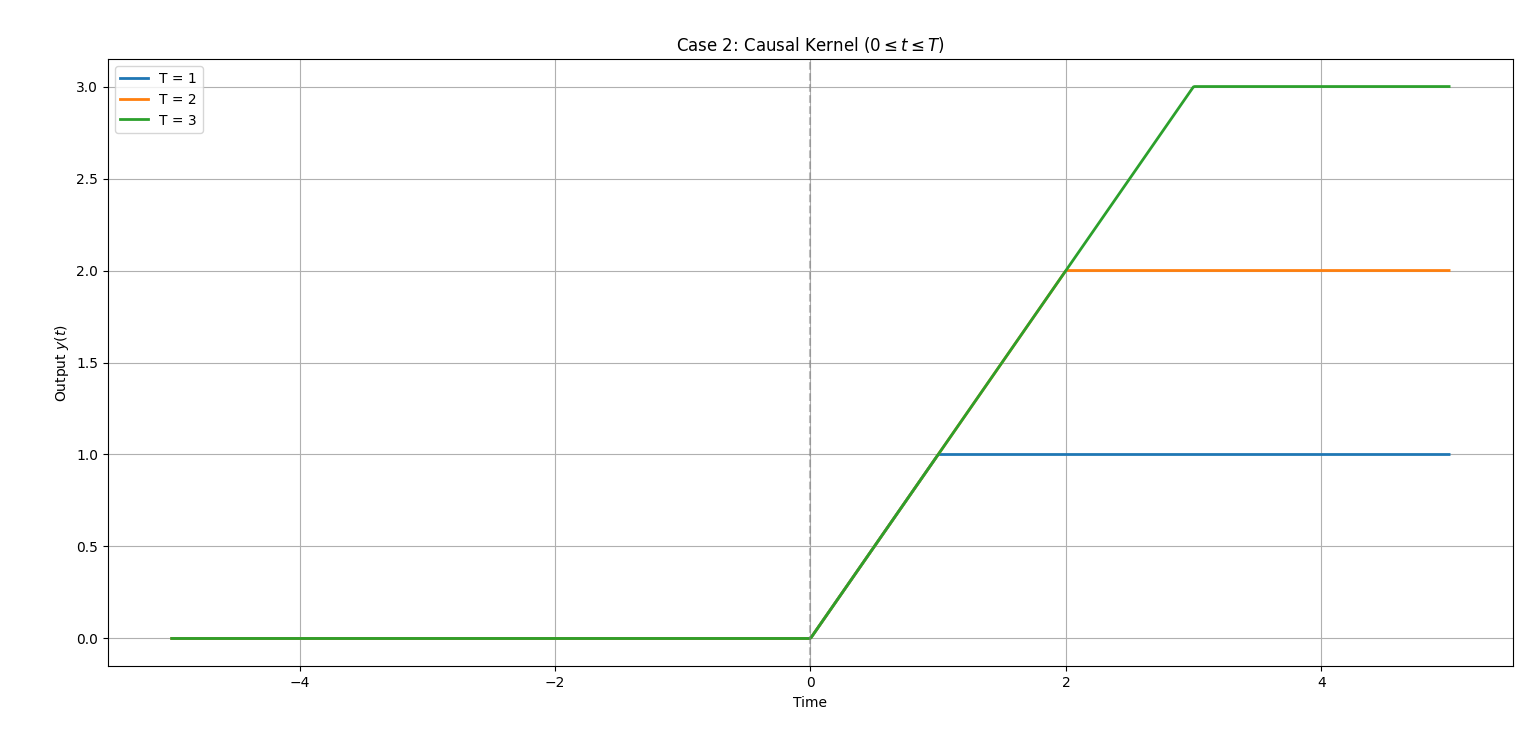
\includegraphics[width=0.8\linewidth]{codes/codes_step/plotsstep/case2step.png}
    \caption{Modified kernel}
    \label{fig:enter-label}
\end{figure}
\subsubsection{Comparison with Original Kernel:}
\begin{itemize}
    \item The response is now \textbf{causal} (output depends only on past/current inputs).
    \item The ramp is shorter (from \( 0 \) to \( T \)) compared to the original (\( -T \) to \( T \)).
    \item The steady-state value is \( T \) instead of \( 2T \).
\end{itemize}

\subsubsection{Shifted Kernel by \( \tau_0 \) (Part b)}

The shifted kernel is:
\begin{equation}
h_{shift}(t) = 
\begin{cases} 
1, & -T + \tau_0 \leq t \leq T + \tau_0 \\
0, & \text{otherwise}
\end{cases}
\end{equation}

Applying the time-shift property of convolution:
\begin{align}
f(t) * h(t-\tau_0) = (f(t) * h(t))_{t \rightarrow t-\tau_0}
\end{align}

The convolution output is simply the original \( y(t) \) delayed by \( \tau_0 \):

\begin{equation}
y_{shift}(t) = y(t - \tau_0) = 
\begin{cases} 
0, & t < -T + \tau_0 \\
(t - \tau_0) + T, & -T + \tau_0 \leq t \leq T + \tau_0 \\
2T, & t > T + \tau_0 
\end{cases}
\end{equation}
\begin{figure}[H]
    \centering
    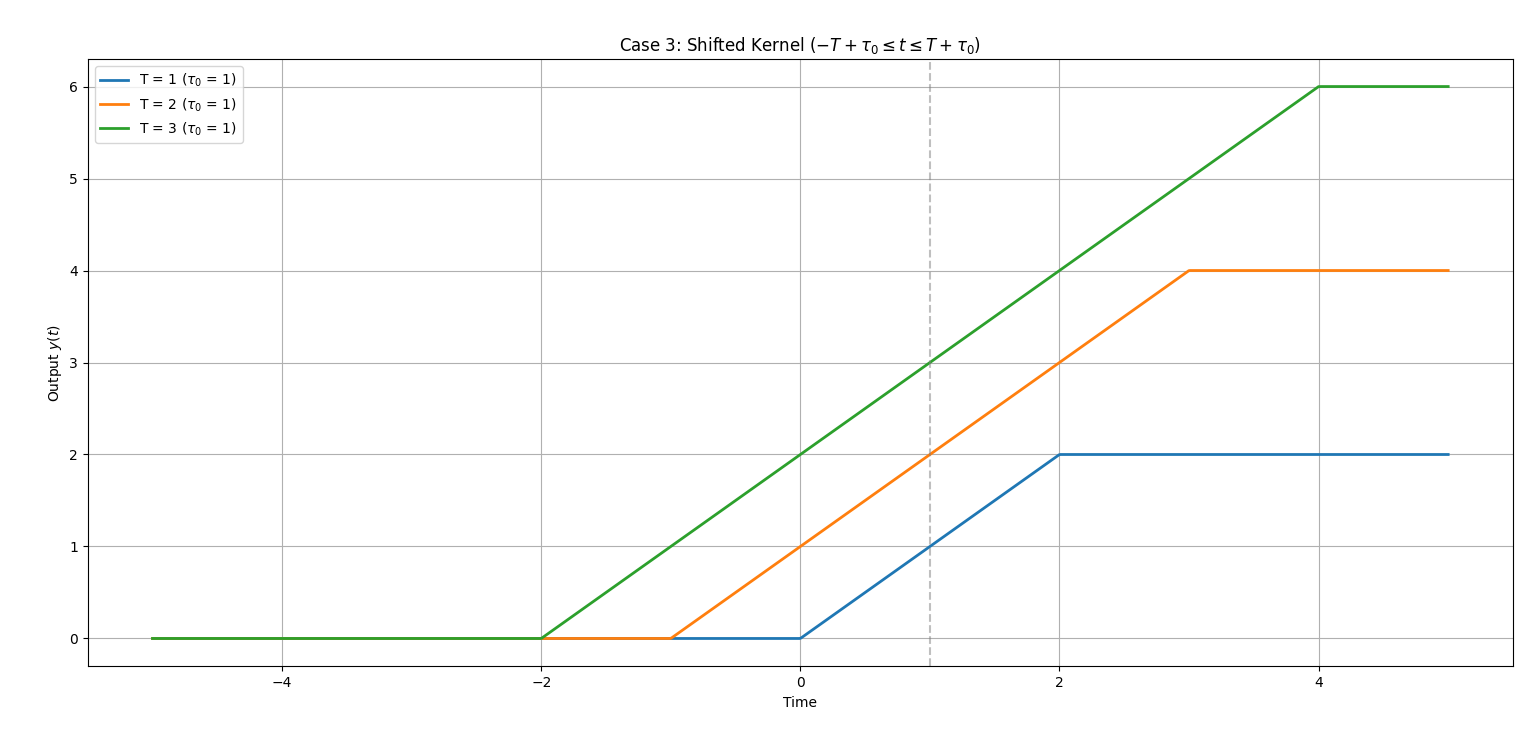
\includegraphics[width=0.8\linewidth]{codes/codes_step/plotsstep/case3step.png}
    \caption{shifted kernel}
    \label{fig:enter-label}
\end{figure}

\subsubsection{Significance in Time-Delayed Systems:}
\begin{itemize}
    \item The shift \( \tau_0 \) introduces a \textbf{time delay} in the system's response.
    \item For \( \tau_0 > 0 \), the response is delayed (system responds later).
    \item For \( \tau_0 < 0 \), the response is advanced (system responds earlier).
    \item Important in control systems, signal processing, and communications where delays affect stability and synchronization.
\end{itemize}

\subsection{Conclusion}

\begin{itemize}
    \item The convolution of a step function with a rectangular kernel produces a \textbf{piecewise linear} output.
    \item Modifying the kernel to be \textbf{causal} changes the response to depend only on past inputs.
    \item Shifting the kernel introduces a \textbf{time delay}, which is crucial in real-world systems.
    \item The kernel width \( T \) directly affects the steady-state value and transition time of the output.
\end{itemize}

This analysis demonstrates how different kernel modifications affect signal processing outcomes and provides insight into the behavior of linear time-invariant systems.
\subsubsection{Comparision of all cases}
\begin{figure}[H]
    \centering
    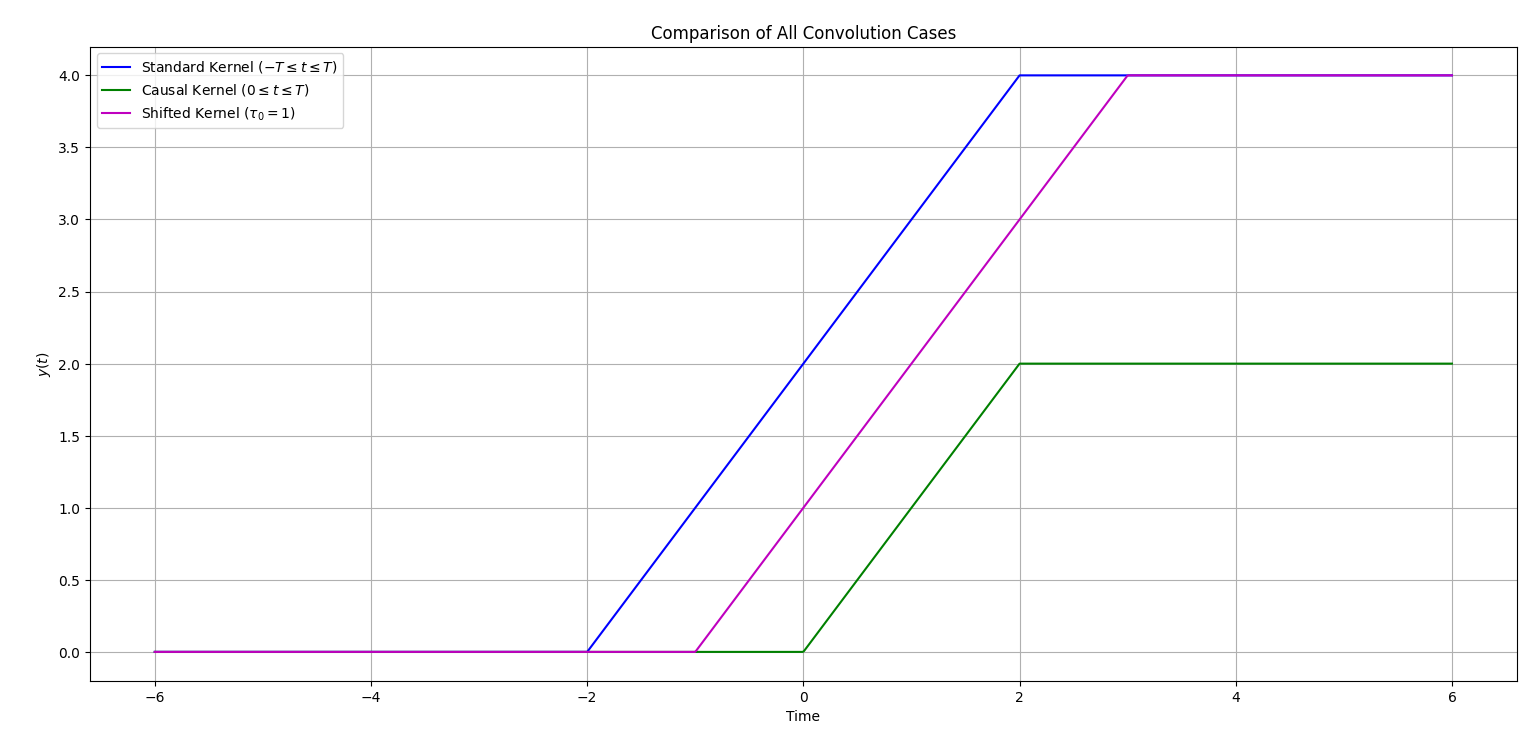
\includegraphics[width=0.8\linewidth]{codes/codes_step/plotsstep/comparsionof123.png}
    \caption{Comparision of all cases}
    \label{fig:enter-label}
\end{figure}
